% GENERATED by tools/make_results.py -- do not edit by hand.
\begin{figure}[t]
\centering
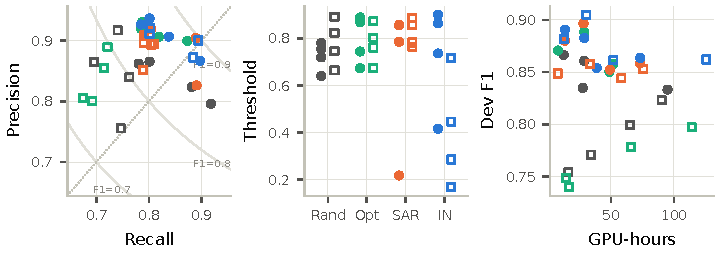
\includegraphics[width=\textwidth]{figures/operating_points}
\caption{Final-evaluation operating points for all 32 cells (filled circles:
ViT; open squares: CNN; colors as in Fig.~\ref{fig:label-efficiency}). Left:
precision--recall positions with iso-F1 contours; most cells sit above the
dotted $P=R$ diagonal. Center: swept threshold by initialization role.
Right: best-development F1 against measured GPU-hours per cell.}
\label{fig:operating-points}
\end{figure}
